\documentclass{beamer}
%\usetheme{kth}
%\usetheme{CambridgeUS}
%\usecolortheme{beaver}
\usepackage[utf8]{inputenc}
\usepackage[european, arrowmos]{circuitikz}
\usepackage{tikz}
 \usetikzlibrary{shapes, calc, intersections, positioning, external}
 \tikzexternalize[prefix=img/extern/]
\usepackage{pgfplots}
 \pgfplotsset{compat=1.15}
 \usepgfplotslibrary{groupplots,fillbetween}
\usepackage{tikz-timing}
\usepackage{siunitx}
\usepackage{amsmath}
\usepackage{amssymb}
\usepackage{amsfonts}
\usepackage{subcaption}
\usepackage{booktabs}
\usepackage{multicol}
\usepackage{minted}

\newcommand*{\subb}[1]{\ensuremath{_{\mathrm{#1}}}}
\newcommand*{\supp}[1]{\ensuremath{^{\mathrm{#1}}}}
\renewcommand*{\j}{\ensuremath{{\mathrm{j}}}}

\addtobeamertemplate{navigation symbols}{}{%
 \usebeamerfont{footline}%
 \usebeamercolor[fg]{footline}%
 \hspace{1em}%
 \raisebox{1.2pt}[0pt][0pt]{\insertframenumber/\inserttotalframenumber}
}

\title{IL2239 - Course Project}
\subtitle{Design of a SAR ADC}
\author{J.~Altayó \and B.~Sunedahl}
\date{March of 2019}

\begin{document}
 \section*{}
 \begin{frame}[plain, t]
  \titlepage
 \end{frame}
 
 \begin{frame}{Outline}
  \begin{multicols}{2}
   \tableofcontents
  \end{multicols}
 \end{frame}
 \section{Project Description}
 \begin{frame}{Project Description}
  Design of a single-ended SAR ADC with the following specifications.
  \begin{itemize}
   \item Comparator clock frequency: \SI{100}{\MHz}
   \item SNDR \textgreater\ 28 dB and SFDR \textgreater\ 37 dB
   \item Technology: \SI{150}{\nm} CMOS
   \item Supply voltage: 1.8 V
   \item Input amplitude ($V\subb{in}$): \SI{0.5}{\volt_{pp}}
   \item Input common-mode voltage: $0 \leq V\subb{in,cm} \leq 1.8$ V
   \item Voltage reference: $V\subb{ref} \leq 1.8$ V
   \item Switching energy below \SI{30}{\pico\joule} for $V\subb{in}=\SI{300}{\mV}$
  \end{itemize}
 \end{frame}
 
 \section{Roles and Responsibilities}
 \begin{frame}{Roles and Responsibilities}
  \begin{columns}
   \begin{column}{0.5\textwidth}
    Jordi:
    \begin{itemize}
     \item Comparator
     \item Successive Approximation Register
     \item Comparator Layout
    \end{itemize}
   \end{column}
   \begin{column}{0.5\textwidth}
    Björn:
    \begin{itemize}
     \item Digital-to-Analog Converter
     \item Sample \& Hold
     \item DAC Layout
    \end{itemize}
   \end{column}
  \end{columns}
 \end{frame}
 \section{Design Flow}
 \begin{frame}{Design Flow}
  We used a top-down design approach:
  \vspace{2em}
  \begin{enumerate}
   \item System-level design
   \item Behavioral modeling using Verilog-AMS
   \item Transistor level modeling
   \item Layout
  \end{enumerate}
  \vspace{2em}
  \visible<2->{Co-simulations where also used to test individual blocks functionality}
%  \begin{center}
%   \resizebox{\textwidth}{!}{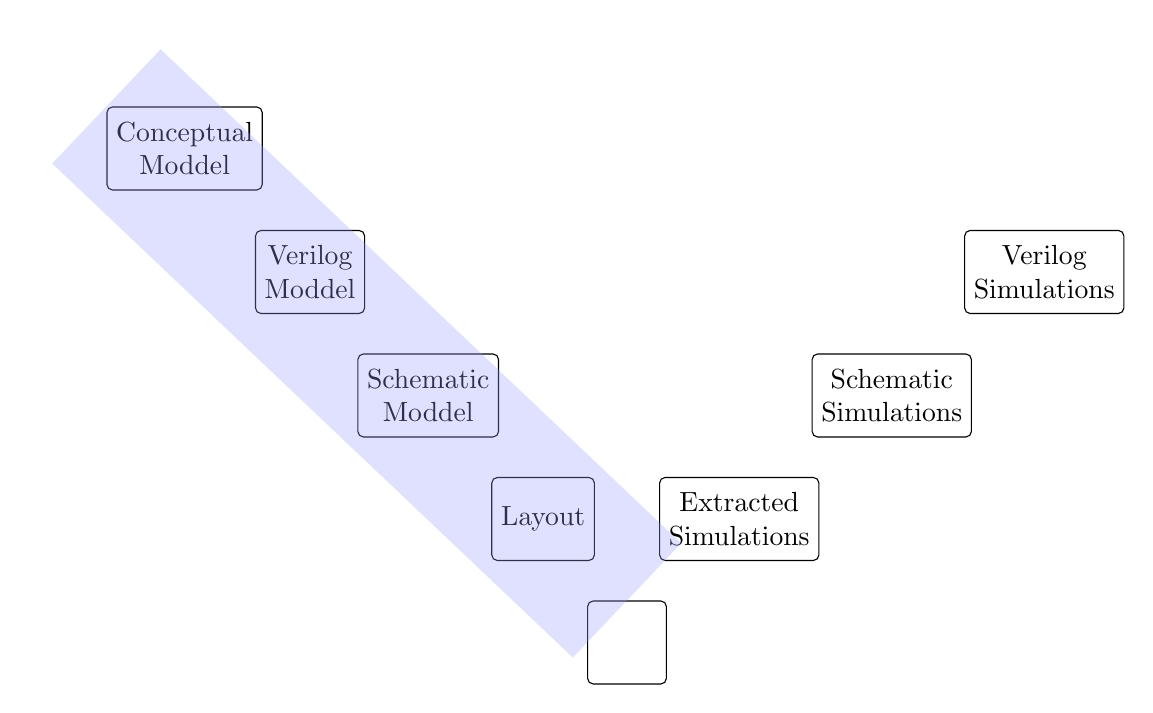
\begin{tikzpicture}[node distance=0.5cm and -0.1cm,every node/.style={align=center,draw, rectangle,rounded corners=2pt, minimum height=3em,}]
 \node (con) {Conceptual\\Moddel};
 \node[below right = of con] (v) {Verilog\\Moddel};
 \node[below right = of v] (sch) {Schematic\\Moddel};
 \node[below right = of sch] (ly) {Layout};
 \node[, minimum width = 1cm, below right = of ly] (en) {};
 \node[above right = of en] (lysim) {Extracted\\Simulations};
 \node[above right = of lysim] (schsim) {Schematic\\Simulations};
 \node[above right = of schsim] (vsim) {Verilog\\Simulations};
 \draw[line width= 2cm, blue!40, opacity=0.3] (con.north west)--(en.north); 
\end{tikzpicture}
}
%  \end{center}
 \end{frame}
 
 \AtBeginSection[]{
  \begin{frame}{Outline}
   \begin{multicols}{2}
    \tableofcontents[
     sectionstyle=show/shaded,
     subsectionstyle=show/show/shaded,
     subsubsectionstyle=show/show/show/shaded
    ]
   \end{multicols}
  \end{frame}
 }

 \section{System-level Design}
 \subsection{Problem Statement}
 \begin{frame}
  {System-level Design I}{Problem Statement}
  The basic block diagram of a SAR ADC looks as follows

  \vspace*{2em}
  \tikzsetnextfilename{sar}
  \resizebox{\textwidth}{!}{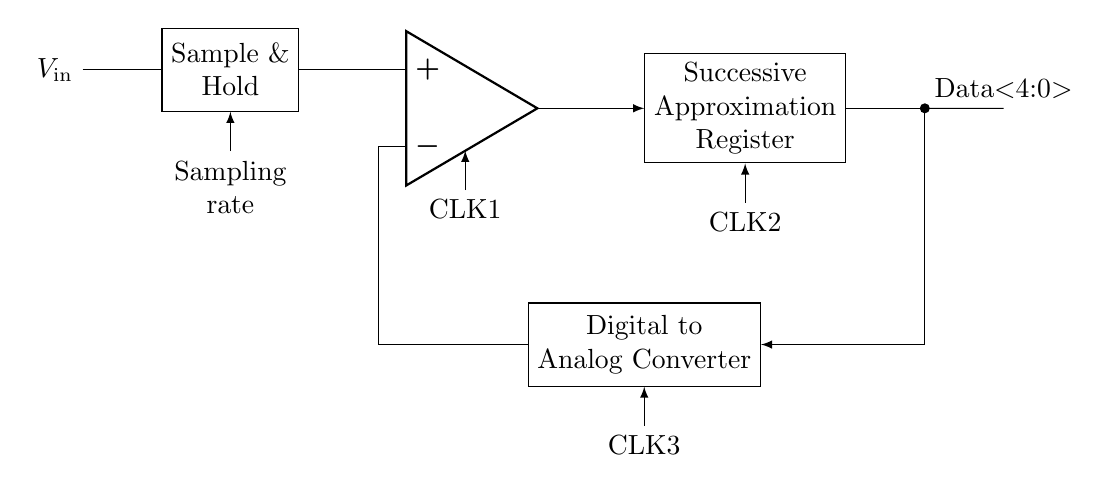
\begin{tikzpicture}
 \draw (0,0) node[left] {$V\subb{in}$} --++ (1,0) node[draw, rectangle, minimum height=3em, anchor=west, align=center] (sh) {Sample \&\\Hold};
 \draw (sh.east) --++ (1,0) node[op amp, noinv input up, anchor=+] (opamp) {};
 \draw[-latex] (opamp.out) --++ (1,0) node[draw, rectangle, minimum height=3em, anchor=west, align=center] (sar) {Successive\\Approximation\\Register};
 %\draw (sar.east) --++ (1,0) --++ (0,-2) coordinate (a) to[dac,>] (a-|opamp.-) -- (opamp.-);
 \draw[-latex] (sar.west)++(0,-3) node[draw, rectangle, minimum height=3em, align=center] (dac) {Digital to\\Analog Converter} (sar.east) --++ (1,0) |- (dac.east);
 \draw (dac.west) -| (opamp.-);
 \draw (sar.east) ++ (1,0) to[short,*-] ++ (1,0) node[above] {Data\textless 4:0\textgreater};
 
 \draw[-latex] (sh.south) ++ (0,-0.5) node[below, align=center] {Sampling\\rate} -- (sh.south);
 \draw[-latex] (opamp.down) ++ (0,-0.5) node[below] {CLK1} -- (opamp.down);
 \draw[-latex] (sar.south) ++ (0,-0.5) node[below] {CLK2} -- (sar.south);
 \draw[-latex] (dac.south) ++ (0,-0.5) node[below] {CLK3} -- (dac.south);
 %\draw[-latex] (7.4,-2.99) ++ (0,-0.5) node[below] {CLK3} --++ (0,0.5);
\end{tikzpicture} 
}
 \end{frame}
 \subsection{Proposed Solution}
 \begin{frame}
  {System-level Design II}{Proposed Solution}
  The following topology was used:
  \vspace{1em}
  \begin{itemize}
   \item Comparator: \alert{Strong ARM Latch}
    \begin{itemize}
     \item[--] Reduced power consumption 
     \item[--] Fast operation
     \item[--] Small area
    \end{itemize}
   \item<2-> DAC: \alert{Charge redistribution weighted capacitors}
    \begin{itemize}
     \item[--] Suitable for CMOS technology
     \item[--] Integrates the Sample \& Hold
    \end{itemize}
   \item<3-> SAR: \alert{Successive Approximation Register}
    \begin{itemize}
     \item[--] Integrates controls for Sample \& Hold
     \item[--] Implemented as 7 state FSM
     \item[--] Verilog model
    \end{itemize}
  \end{itemize}
 \end{frame}
 \subsection{Behavioral Modeling}
 \subsubsection{Comparator}
 \begin{frame}[fragile]{System-level Design III}{Behavioral Modeling I}
  Comparator modeling:\vspace{-1ex}
  \begin{minted}%{verilog}
   [
    frame=lines,
    framesep=2mm,
    baselinestretch=1.2,
    fontsize=\footnotesize,
    linenos
   ]{verilog}
always @(posedge CLK) begin
    #5
    outn = 0; outp = 0;
end
always @(negedge CLK) begin
  if(V(inp) > V(inn)) begin
    #50
    outp = 1; outn = 0;
  end else begin
    #50
    outp = 0; outn = 1;
  end
end
  \end{minted}
  Some delay was added to the behavioral model.
 \end{frame}

 \subsubsection{Digital-to-Analog Converter}
 \begin{frame}[fragile]{System-level Design III}{Behavioral Modeling II}
  Digital-to-Analog Converter modeling:
  \begin{minted}%{verilog}
   [
    frame=lines,
    framesep=2mm,
    baselinestretch=1.2,
    fontsize=\footnotesize,
    linenos
   ]{verilog}
analog begin
  always @(posedge CLK) begin
    for(i=0, i < 5, i++) begin
      result += input[5-i] * Vref/(1<<i);
    end
    V(out) <+ transition(result, 1ns, 0.1ns, 0.1ns)
  end
end
  \end{minted}
 \end{frame}
 \subsubsection{Successive Approximation Register}
 \begin{frame}{System-level Design III}{Behavioral Modeling III}
  SAR algorithm: binary search\hspace*{1em}
  \begin{columns}
   \begin{column}{0.5\textwidth}
    \tikzexternaldisable
    \tikzsetnextfilename{sar_algorithm}
    \resizebox{!}{0.7\textheight}{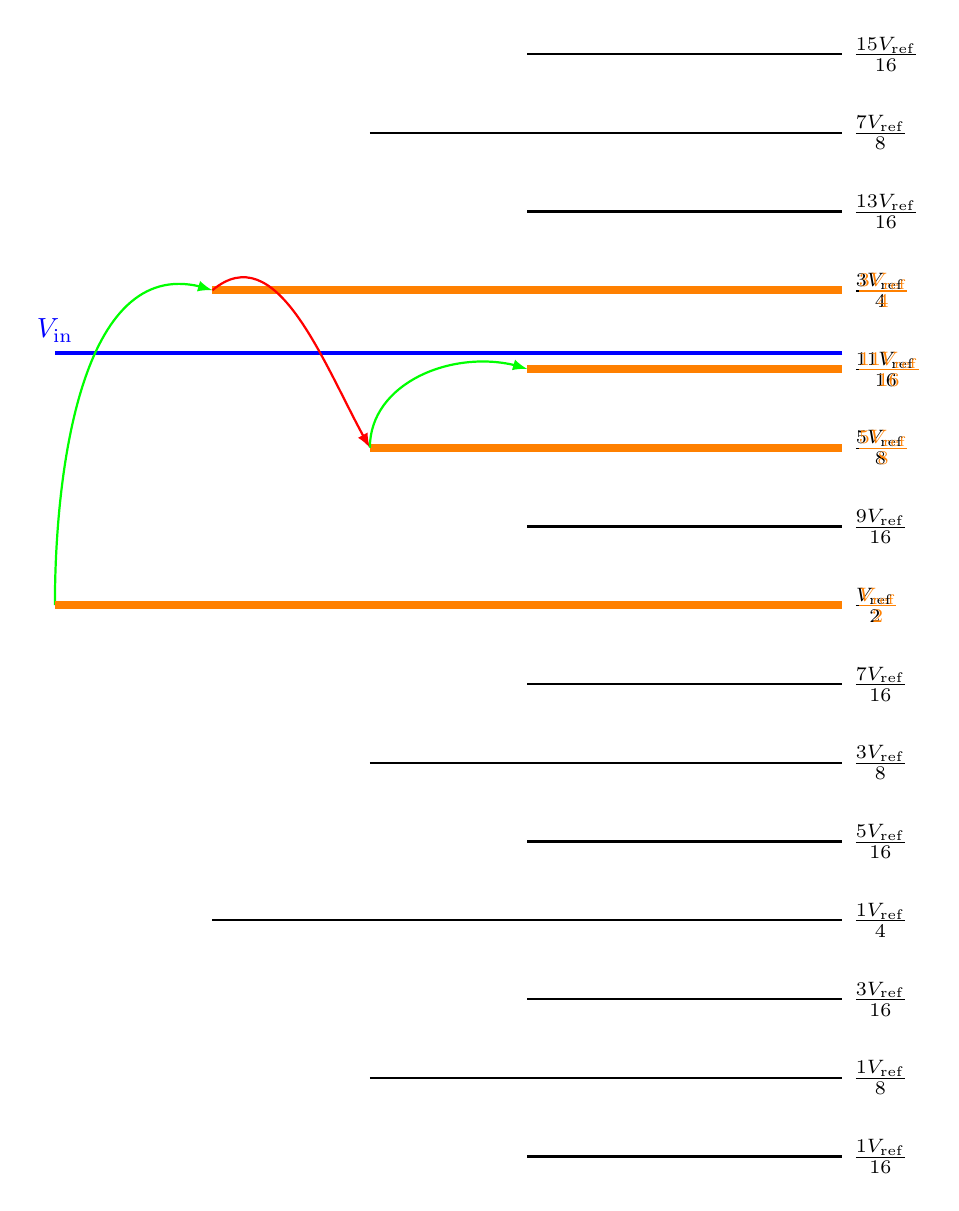
\begin{tikzpicture}
 \draw[thick] (0, 0) --++ (10,0) node[right]{$\frac{V\subb{ref}}{2}$};
 \draw[thick] (2, 4) --++ (8,0) node[right]{$\frac{3V\subb{ref}}{4}$};
 \draw[thick] (2,-4) --++ (8,0) node[right]{$\frac{1V\subb{ref}}{4}$};
 \draw[thick] (4, 6) --++ (6,0) node[right]{$\frac{7V\subb{ref}}{8}$};
 \draw[thick] (4,-6) --++ (6,0) node[right]{$\frac{1V\subb{ref}}{8}$};
 \draw[thick] (4,-2) --++ (6,0) node[right]{$\frac{3V\subb{ref}}{8}$};
 \draw[thick] (4, 2) --++ (6,0) node[right]{$\frac{5V\subb{ref}}{8}$};
 \draw[thick] (6, 1) --++ (4,0)  node[right]{$\frac{9V\subb{ref}}{16}$};
 \draw[thick] (6, 3) --++ (4,0)  node[right]{$\frac{11V\subb{ref}}{16}$};
 \draw[thick] (6, 5) --++ (4,0)  node[right]{$\frac{13V\subb{ref}}{16}$};
 \draw[thick] (6, 7) --++ (4,0)  node[right]{$\frac{15V\subb{ref}}{16}$};
 \draw[thick] (6, -1) --++ (4,0) node[right]{$\frac{7V\subb{ref}}{16}$};
 \draw[thick] (6, -3) --++ (4,0) node[right]{$\frac{5V\subb{ref}}{16}$};
 \draw[thick] (6, -5) --++ (4,0) node[right]{$\frac{3V\subb{ref}}{16}$};
 \draw[thick] (6, -7) --++ (4,0) node[right]{$\frac{1V\subb{ref}}{16}$};
 \draw[line width = 0.05cm, blue] (10, 3.2) --++(-10,0) node[above] {$V\subb{in}$};
 \visible<2->{\draw[-latex, thick, green] (0,0) to[out=90, in=160] (2,4);}
 \visible<2>{\draw[line width=0.1cm, orange] (0, 0) --++ (10,0) node[right]{$\frac{V\subb{ref}}{2}$};}
 \visible<3>{\draw[line width=0.1cm, orange] (2, 4) --++ (8,0) node[right]{$\frac{3V\subb{ref}}{4}$};}
 \visible<4>{\draw[line width=0.1cm, orange] (4, 2) --++ (6,0) node[right]{$\frac{5V\subb{ref}}{8}$};}
 \visible<5>{\draw[line width=0.1cm, orange] (6, 3) --++ (4,0) node[right]{$\frac{11V\subb{ref}}{16}$};}
 \visible<3->{\draw[-latex, thick, red] (2,4) to[out=40, in=120] (4,2);}
 \visible<4->{\draw[-latex, thick, green] (4,2) to[out=90, in=160] (6,3);}
\end{tikzpicture}
}
   \end{column}
   \begin{column}{0.5\textwidth}
    Assume $V\subb{in}=\SI{0.7}{\V}$, $V\subb{ref}=\SI{1}{\V}$ and 4 bits\vspace{1em}
    \begin{enumerate}
     \item<2-> $V\subb{in} \overset{?}{\ge} \frac{V\subb{ref}}{2}$ {\color{green}\checkmark}
     \item<3-> $V\subb{in} \overset{?}{\ge} \frac{3V\subb{ref}}{4}$ {\color{red}\text{\sffamily X}}
     \item<4-> $V\subb{in} \overset{?}{\ge} \frac{5V\subb{ref}}{8}$ {\color{green}\checkmark}
     \item<5-> $V\subb{in} \overset{?}{\ge} \frac{11V\subb{ref}}{16}$ {\color{green}\checkmark}
    \end{enumerate}
    \vspace{2em}
    \visible<6->{Out = 0b1011 ($\frac{11V\subb{ref}}{16}$)}

   \end{column}
  \end{columns}
 \end{frame}
 \section{Transistor-level Design}
 \subsection{Comparator}
 \begin{frame}{Transistor-level Design I}{Comparator}
  Strong ARM Latch topology\par\vspace{1em}
  \resizebox{\textwidth}{!}{\centering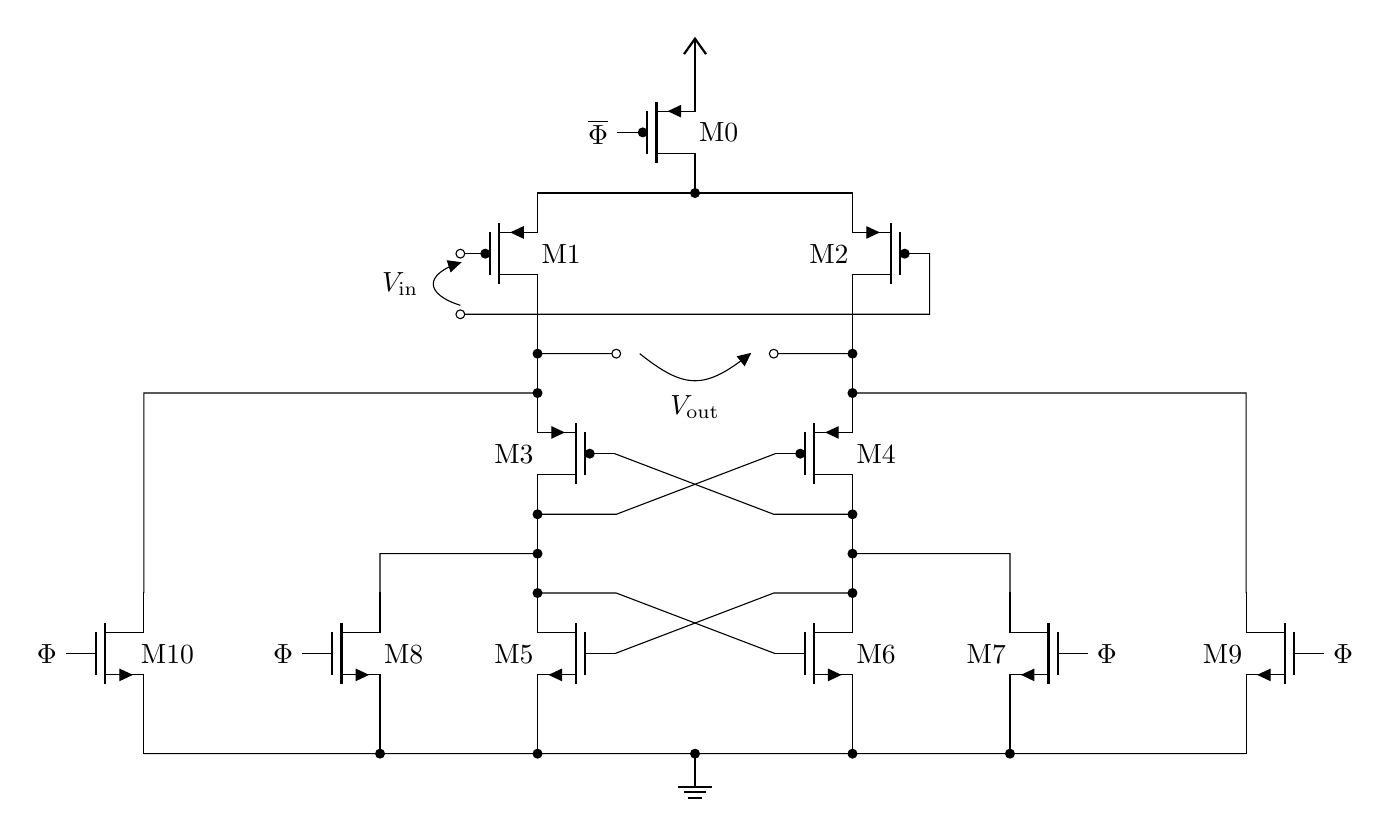
\begin{tikzpicture}
 \draw node[vcc]{} node[pmos, anchor=S] (M0){};
 \draw (M0.D) --++ (-2,0) node[pmos, anchor=S] (M1){};
 \draw (M0.D) to[short, *-] ++ (2,0)  node[pmos, xscale=-1, anchor=S] (M2){};
 \draw (M1.D) --++ (0,-1) node[pmos, anchor=S, xscale=-1] (M3){};
 \draw (M2.D) --++ (0,-1) node[pmos, anchor=S] (M4){};
 \draw (M3.D) --++ (0,-1) node[nmos, anchor=D, xscale=-1] (M5){};
 \draw (M4.D) --++ (0,-1) node[nmos, anchor=D] (M6){};
 \draw (M3.G) -- ($(M4.D)-(1,0)$) to[short,-*] (M4.D);
 \draw (M4.G) -- ($(M3.D)+(1,0)$) to[short,-*] (M3.D);
 \draw (M5.G) -- ($(M6.D)-(1,0)$) to[short,-*] (M6.D);
 \draw (M6.G) -- ($(M5.D)+(1,0)$) to[short,-*] (M5.D);
 \draw (M2.G) |- (M2.D) coordinate (en) -- (en-|M1.G) to[open, o-o, v^=$V\subb{in}$] (M1.G);
 \draw (M6.D) ++ (0,0.5) to[short, *-] ++(2,0) --++ (0,-0.5) node[nmos, anchor=D, xscale=-1] (M7) {};
 \draw (M5.D) ++ (0,0.5) to[short, *-] ++(-2,0) --++ (0,-0.5) node[nmos, anchor=D] (M8) {};
 \draw (M4.S) to[short, *-] ++(5,0) coordinate(aa) -- (aa|-M7.D) node[nmos, anchor=D, xscale=-1] (M9) {};
 \draw (M3.S) to[short, *-] ++(-5,0) coordinate(aaa) -- (aaa|-M7.D) node[nmos, anchor=D] (M10) {};
 \draw (M1.D) ++ (0,-0.5) to[short, *-] ++(1,0) coordinate (op);
 \draw (M2.D) ++ (0,-0.5) to[short, *-] ++(-1,0) coordinate (on);
 \draw (op) to[open, o-o, v=$V\subb{out}$] (on);
 \draw (M9.S) --++ (0,-0.5) (M5.S) --++ (0,-0.5) (M6.S) --++ (0,-0.5) (M7.S) --++ (0,-0.5) (M8.S) --++ (0,-0.5) (M10.S) --++ (0,-0.5);
 \draw (M10.S) ++ (0,-0.5) to[short,-*] ++(3,0) to[short,-*] ++(2,0) to[short,-*] ++(4,0) to[short,-*] ++(2,0) to[short] ++(3,0);
 \draw ($0.5*(M5.S) + 0.5*(M6.S)$) ++ (0,-0.5) node[ground] {} node[circ]{};

 \draw (M0) ++ (0.3,0) node[]{M0}; 
 \draw (M1) ++ (0.3,0) node[]{M1}; 
 \draw (M2) ++ (-0.3,0) node[]{M2}; 
 \draw (M3) ++ (-0.3,0) node[]{M3}; 
 \draw (M4) ++ (0.3,0) node[]{M4}; 
 \draw (M5) ++ (-0.3,0) node[]{M5}; 
 \draw (M6) ++ (0.3,0) node[]{M6}; 
 \draw (M7) ++ (-0.3,0) node[]{M7}; 
 \draw (M8) ++ (0.3,0) node[]{M8}; 
 \draw (M9) ++ (-0.3,0) node[]{M9}; 
 \draw (M10) ++ (0.3,0) node[]{M10}; 

 \draw (M0.G) node[left] {$\overline{\Phi}$};
 \draw (M7.G) node[right] {$\Phi$};
 \draw (M8.G) node[left]  {$\Phi$};
 \draw (M9.G) node[right] {$\Phi$};
 \draw (M10.G) node[left] {$\Phi$};
\end{tikzpicture}
}
  %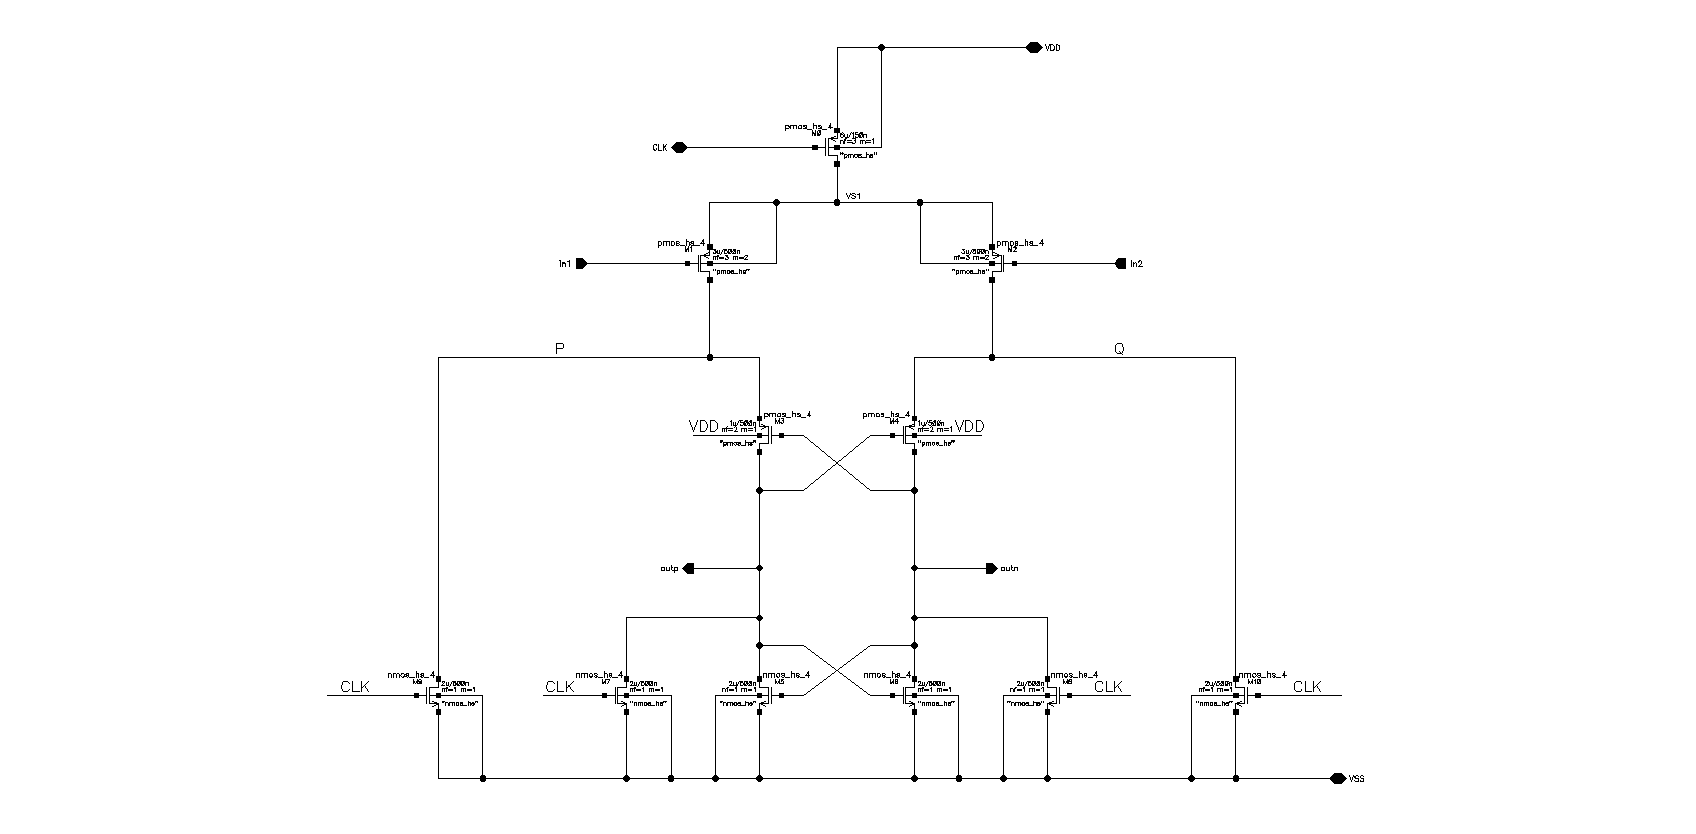
\includegraphics[width=0.9\textwidth]{img/comp_sch}
 \end{frame}
 \subsection{Digital-to-Analog Converter}
 \begin{frame}{Transistor-level Design II}{Digital-to-Analog Converter I}
  Example with 3 bit\vspace*{1em}
  \begin{center}
   \resizebox{\textwidth}{!}{\begin{tikzpicture}
 \draw (0,0) to[C,l=$4C$] ++(0,-2);
 \draw (4,0) to[C,l=$2C$] ++(0,-2);
 \draw (8,0) to[C,l=$C$] ++(0,-2);
 \draw (12,0) to[C,l=$C$] ++(0,-2);

 \draw (0,-2) --++ (-1,0) node[nmos,anchor=D,xscale=-1] (M1) {};
 \draw (0,-2) to[short,*-] ++ (1,0) node[nmos,anchor=D,xscale=-1] (M2) {};
 \draw (4,-2) --++ (-1,0) node[nmos,anchor=D,xscale=-1] (M3) {};
 \draw (4,-2) to[short,*-] ++ (1,0) node[nmos,anchor=D,xscale=-1] (M4) {};
 \draw (8,-2) --++ (-1,0) node[nmos,anchor=D,xscale=-1] (M5) {};
 \draw (8,-2) to[short,*-] ++ (1,0) node[nmos,anchor=D,xscale=-1] (M6) {};
 \draw (12,-2) --++ (-1,0) node[nmos,anchor=D,xscale=-1] (M7) {};
 \draw (12,-2) to[short,*-] ++ (1,0) node[nmos,anchor=D,xscale=-1] (M8) {};
 \draw (M8.S) --++(0,-1) to[short,-*] ++(-4,0) to[short,-*] ++(-4,0) to[short] ++(-4,0) --++(0,1) (M4.S) --++ (0,-1) (M6.S) --++(0,-1);
 \draw (M7.S) to[short,-*] ++(-4,0) to[short,-*] ++(-4,0) to[short,-*] ++(-4,0) to[short,-o] ++(-1,0) node[left]{$V\subb{SS}$};
 \draw (M3.S) ++ (0,-1) to[short,*-] ++(0,-1) node[nmos,anchor=D] (M9) {} (M9.S) to[short, -o] ++ (0,-.1) node[below] {$V\subb{ref}$};
 \draw (M5.S) ++ (0,-1) to[short,*-] ++(0,-1) node[nmos,anchor=D, xscale=-1] (M10) {} (M10.S) to[short, -o] ++(0,-.1) node[below] {$V\subb{in}$};
 \draw (0,0) to[short,-*] ++(4,0) to[short,-*] ++(4,0) to[short,-*] ++(4,0) to[short,-o] ++(8,0) coordinate (en) node[right]{$V\subb{out}$};
 \draw (en) ++(-1,0) to[short, *-] ++(0,-2) node[nmos, anchor=D] (M11) {} (M11.S) to[short,-o] ++(0,-1) node[below] {$V\subb{cm}$};

 \draw (M1.G) node[right] {$\overline{\text{b2}}$};
 \draw (M3.G) node[right] {$\overline{\text{b1}}$};
 \draw (M5.G) node[right] {$\overline{\text{b0}}$};
 \draw (M2.G) node[right] {b2};
 \draw (M4.G) node[right] {b1};
 \draw (M6.G) node[right] {b0};
 \draw (M7.G) node[right] {SW\_ref};
 \draw (M8.G) node[right] {SW\_in};
 \draw (M9.G) node[left] {SW\_ref};
 \draw (M10.G) node[right] {SW\_in};
 \draw (M11.G) node[left] {SW\_in};
\end{tikzpicture}
}
  %\makebox[\textwidth][c]{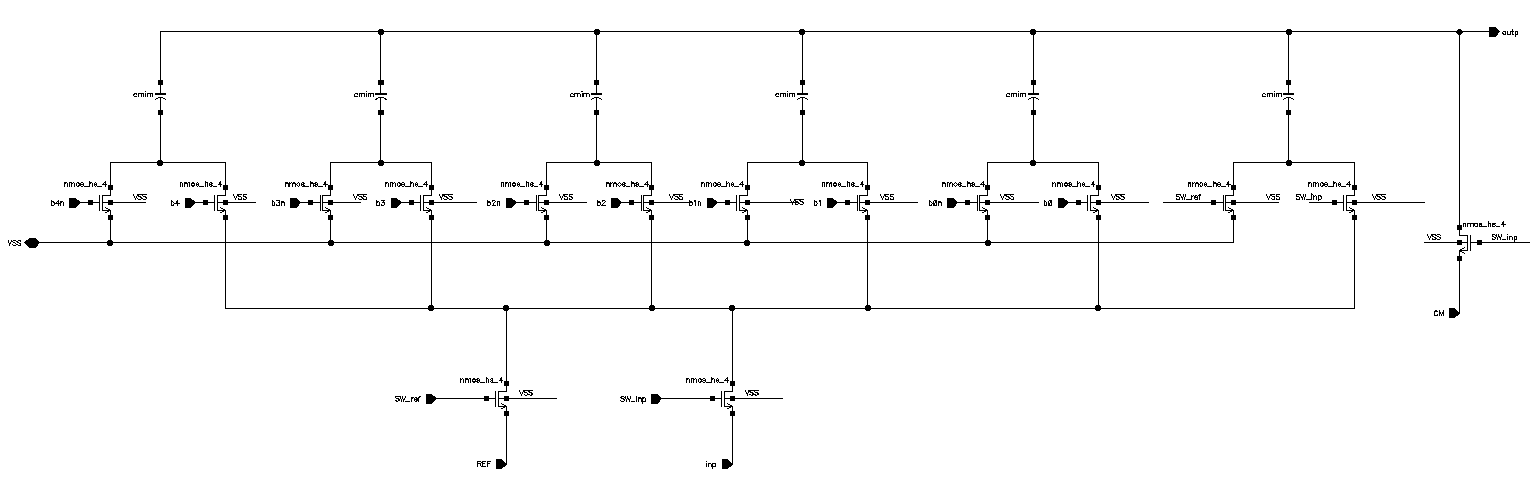
\includegraphics[width=1.1\textwidth]{img/dac_sch}}
  \end{center}
 \end{frame}

 \begin{frame}{Transistor-level Design II}{Digital-to-Analog Converter II}
  Sample phase:
  \vspace*{1em}
  \tikzsetnextfilename{dac_sample}
  \begin{center}
   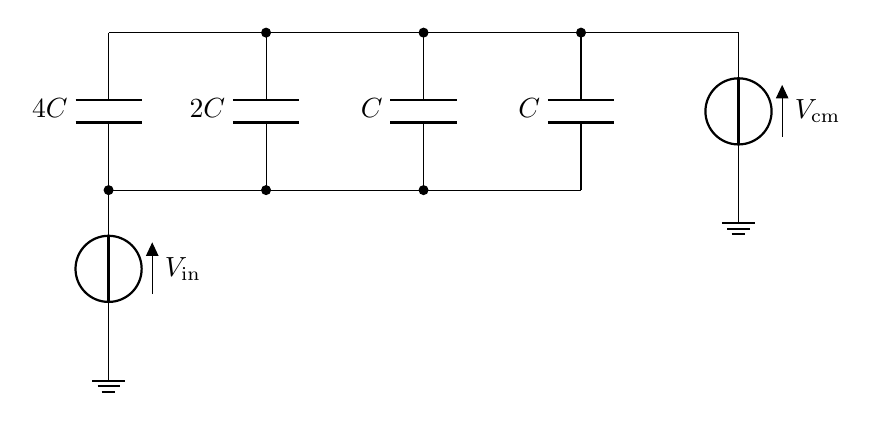
\begin{tikzpicture}
 \draw (0,0) to [C, l=$4C$] ++ (0,2);
 \draw (2,0) to [C, l=$2C$] ++ (0,2);
 \draw (4,0) to [C, l=$C$] ++ (0,2);
 \draw (6,0) to [C, l=$C$] ++ (0,2);
 \draw (0,2) to [short, -*] ++ (2,0) to [short, -*] ++ (2,0) to [short, -*] ++ (2,0) to [short] ++ (2,0);
 \draw (8,2) to [european voltage source, v<=$V\subb{cm}$] ++(0,-2) node [ground] {};
 \draw (0,0) to [short, -*] ++ (2,0) to [short, -*] ++ (2,0) to [short] ++ (2,0);
 \draw (0,0) to [european voltage source, v<=$V\subb{in}$, *-] ++(0,-2) node [ground] {};
\end{tikzpicture}

  \end{center}
 \end{frame}

 \begin{frame}{Transistor-level Design II}{Digital-to-Analog Converter II}
  Cycling phase:\hfill Input word: \alert{0b100}
  \vspace*{1em}
  \tikzsetnextfilename{dac_cycling}
  \begin{center}
   \begin{tikzpicture}
 \draw (0,0) to [C, l=$4C$] ++ (0,2);
 \draw (2,0) to [C, l=$2C$] ++ (0,2);
 \draw (4,0) to [C, l=$C$] ++ (0,2);
 \draw (6,0) to [C, l=$C$] ++ (0,2);
 \draw (0,2) to [short, -*] ++ (2,0) to [short, -*] ++ (2,0) to [short, -*] ++ (2,0) to [short] ++ (2,0);
 \draw (8,2) to [open, o-o, v^<=$V\subb{out}$] ++(0,-2) node [ground] {};
 \draw (0,0) to [european voltage source, v<=$V\subb{ref}$] ++(0,-2) node [ground] {};
 \draw (2,0) to [short, -*] ++ (2,0) to [short, -*] ++ (2,0) node [ground] {};
\end{tikzpicture}

  \end{center}
 \end{frame}

 \begin{frame}{Transistor-level Design II}{Digital-to-Analog Converter II}
  Equivalent circuit:\hfill Input word: \alert{0b100}
  \vspace*{1em}
  \tikzsetnextfilename{dac_equivalent}
  \begin{center}
   \begin{tikzpicture}
 \draw (0,0) node[ground]{} to [C, l=$4C$] ++ (0,2) to [C, l=$4C$] ++ (0,2);
 \draw (0,4) --++ (-3,0) to [european voltage source, v<=$V\subb{ref}$] ++ (0,-4) node [ground]{};
 \draw (0,2) to[short,*-o] ++ (1,0) node[right] {$V\subb{out}=V\subb{cm}-V\subb{in}+\frac{V\subb{ref}}{2}$};
\end{tikzpicture}

  \end{center}
 \end{frame}

 \begin{frame}{Transistor-level Design II}{Digital-to-Analog Converter II}
  Cycling phase:\hfill Input word: \alert{0b010}
  \vspace*{1em}
  \tikzsetnextfilename{dac_cycling2}
  \begin{center}
   \begin{tikzpicture}
 \draw (0,0) to [C, l=$4C$] ++ (0,2);
 \draw (2,0) to [C, l=$2C$] ++ (0,2);
 \draw (4,0) to [C, l=$C$] ++ (0,2);
 \draw (6,0) to [C, l=$C$] ++ (0,2);
 \draw (0,2) to [short, -*] ++ (2,0) to [short, -*] ++ (2,0) to [short, -*] ++ (2,0) to [short] ++ (2,0);
 \draw (8,2) to [open, o-o, v^<=$V\subb{out}$] ++(0,-2) node [ground] {};
 \draw (2,0) to [european voltage source, v<=$V\subb{ref}$] ++(0,-2) node [ground] {};
 \draw (4,0) to [short, -*] ++ (2,0) node [ground] {} (0,0) node[ground]{};
\end{tikzpicture}

  \end{center}
 \end{frame}

 \begin{frame}{Transistor-level Design II}{Digital-to-Analog Converter II}
  Equivalent circuit:\hfill Input word: \alert{0b010}
  \vspace*{1em}
  \tikzsetnextfilename{dac_equivalent2}
  \begin{center}
   \begin{tikzpicture}
 \draw (0,0) node[ground]{} to [C, l=$6C$] ++ (0,2) to [C, l=$2C$] ++ (0,2);
 \draw (0,4) --++ (-3,0) to [european voltage source, v<=$V\subb{ref}$] ++ (0,-4) node [ground]{};
 \draw (0,2) to[short,*-o] ++ (1,0) node[right] {$V\subb{out}=V\subb{cm}-V\subb{in}+\frac{V\subb{ref}}{4}$};
\end{tikzpicture}

  \end{center}
 \end{frame}
%\addtocontents{toc}{\newpage}
 \section{Layout}
 \subsection{Comparator}
 \begin{frame}{Layout I}{Comparator}
  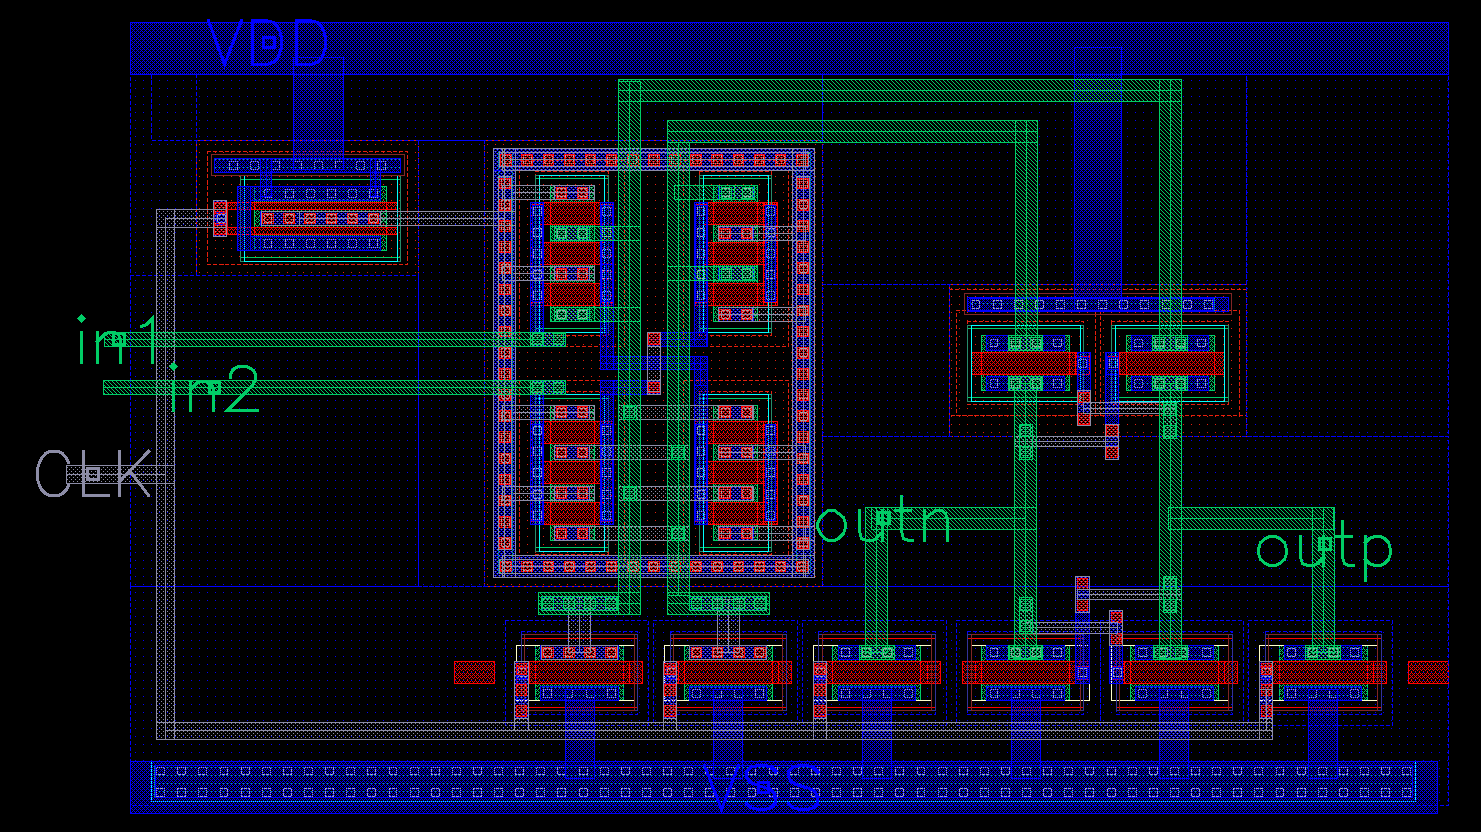
\includegraphics[width=\textwidth]{img/comparator_layout}

  \begin{columns}
   \begin{column}{0.5\textwidth}
    \begin{itemize}
     \item Common centroid for the differential input pair
    \end{itemize}
   \end{column}
   \begin{column}{0.5\textwidth}
    \begin{itemize}
     \item<2-> Guard ring around sensitive high impedance nodes
    \end{itemize}
   \end{column}
  \end{columns}
 \end{frame}
 
 \subsection{Digital-to-Analog Converter}
 \begin{frame}{Layout II}{Digital-to-Analog Converter I}
    \begin{columns}
    \begin{column}{0.40\linewidth}
    To ensure good matching we used: 
    \begin{itemize}
        \item Common centroid technique
        \item<2-> Base unit of half the minmum capacitance
        \item<3-> Dummy capacitors at the edges
    \end{itemize}
    \vspace{3em}
    \end{column}
    \begin{column}{0.60\linewidth}
        \centering
        \tikzsetnextfilename{cap_matrix}
        \resizebox{!}{\textwidth}{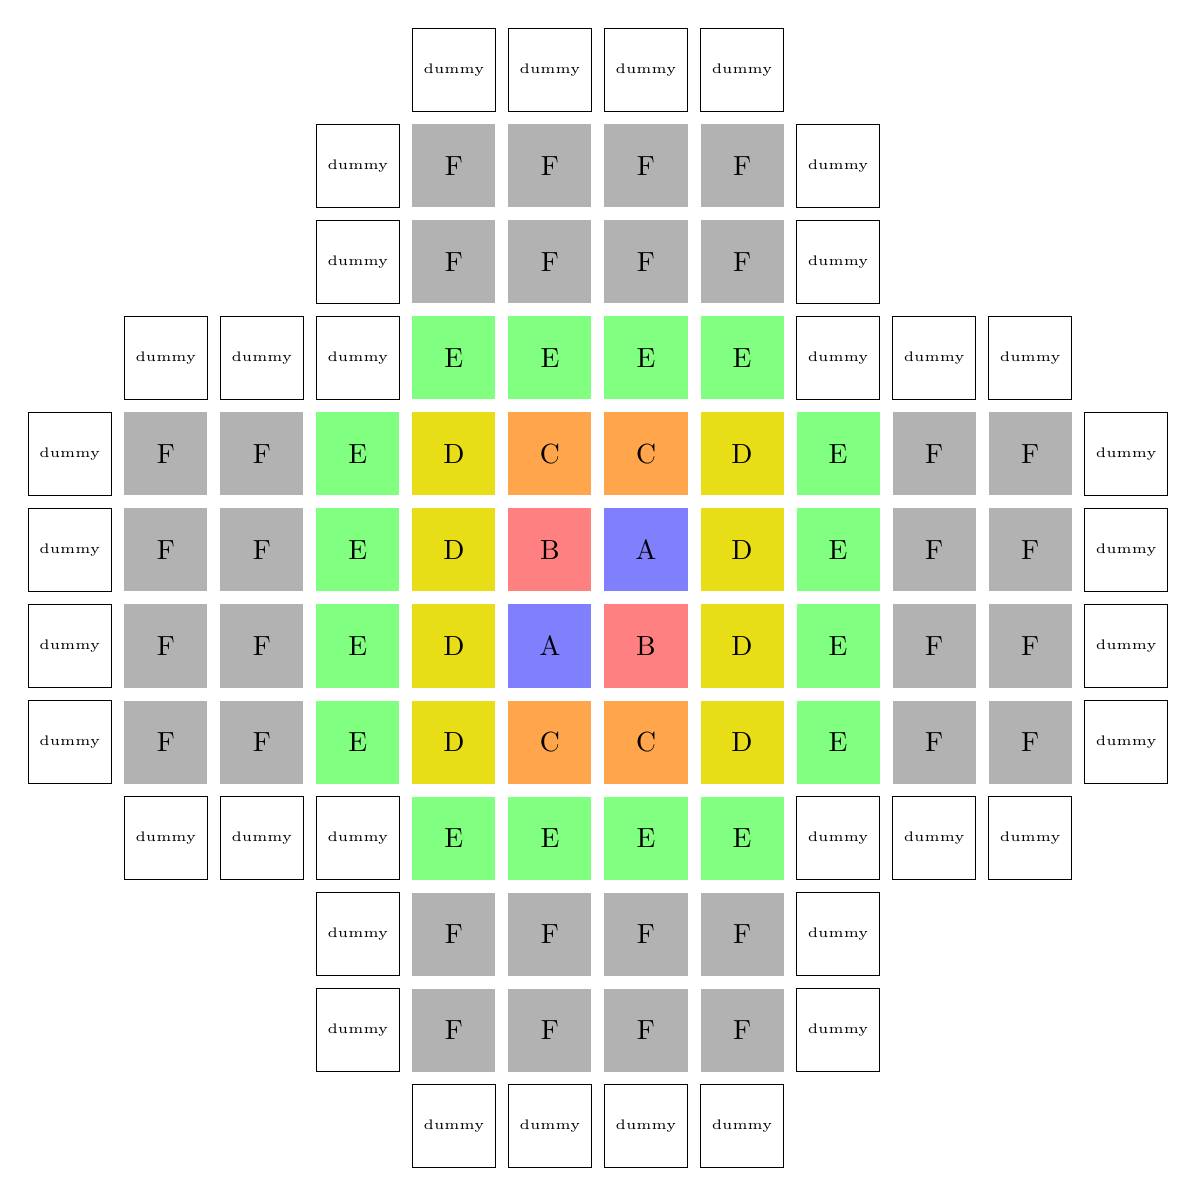
\begin{tikzpicture}[node distance = 1ex]
 \tikzstyle{A} = [fill=blue!50, rectangle, minimum height=3em, minimum width=3em]
 \tikzstyle{B} = [fill=red!50, rectangle, minimum height=3em, minimum width=3em]
 \tikzstyle{C} = [fill=orange!70, rectangle, minimum height=3em, minimum width=3em]
 \tikzstyle{D} = [fill=yellow!90!black, rectangle, minimum height=3em, minimum width=3em]
 \tikzstyle{E} = [fill=green!50, rectangle, minimum height=3em, minimum width=3em]
 \tikzstyle{F} = [fill=black!30, rectangle, minimum height=3em, minimum width=3em]
 \tikzstyle{d} = [draw, rectangle, minimum height=3em, minimum width=3em]
 
 \node [A] (A1) {A};
 \node [B, left  = of A1]  (B1) {B};
 \node [A, below = of B1]  (A2) {A};
 \node [B, below = of A1]  (B2) {B};
 \node [C, below = of A2]  (C1) {C};
 \node [C, below = of B2]  (C2) {C};
 \node [C, above = of A1]  (C3) {C};
 \node [C, above = of B1]  (C4) {C};
 \node [D, left  = of C4]  (D1) {D};
 \node [D, left  = of B1]  (D2) {D};
 \node [D, left  = of A2]  (D3) {D};
 \node [D, left  = of C1]  (D4) {D};
 \node [D, right = of C3]  (D5) {D};
 \node [D, right = of B2]  (D6) {D};
 \node [D, right = of A1]  (D7) {D};
 \node [D, right = of C2]  (D8) {D};
 \node [E, left  = of D1]  (E1) {E};
 \node [E, left  = of D2]  (E2) {E};
 \node [E, left  = of D3]  (E3) {E};
 \node [E, left  = of D4]  (E4) {E};
 \node [E, right = of D5]  (E5) {E};
 \node [E, right = of D6]  (E6) {E};
 \node [E, right = of D7]  (E7) {E};
 \node [E, right = of D8]  (E8) {E};
 \node [E, below = of D8]  (E9) {E};
 \node [E, below = of D4]  (E10) {E};
 \node [E, below = of C2]  (E11) {E};
 \node [E, below = of C1]  (E12) {E};
 \node [E, above = of C3]  (E13) {E};
 \node [E, above = of C4]  (E14) {E};
 \node [E, above = of D1]  (E15) {E};
 \node [E, above = of D5]  (E16) {E};
 \node [F, left  = of E1]  (F1) {F}; 
 \node [F, left  = of E2]  (F2) {F}; 
 \node [F, left  = of E3]  (F3) {F}; 
 \node [F, left  = of E4]  (F4) {F}; 
 \node [F, right = of E5]  (F5) {F}; 
 \node [F, right = of E6]  (F6) {F}; 
 \node [F, right = of E7]  (F7) {F}; 
 \node [F, right = of E8]  (F8) {F}; 
 \node [F, below = of E9]  (F9) {F}; 
 \node [F, below = of E10] (F10) {F}; 
 \node [F, below = of E11] (F11) {F}; 
 \node [F, below = of E12] (F12) {F}; 
 \node [F, above = of E13] (F13) {F}; 
 \node [F, above = of E14] (F14) {F}; 
 \node [F, above = of E15] (F15) {F}; 
 \node [F, above = of E16] (F16) {F}; 
 \node [d, right = of F16] (F17) {\tiny dummy}; 
 \node [d, below = of F17] (F19) {\tiny dummy}; 
 \node [d, right = of F19] (F20) {\tiny dummy}; 
 \node [d, left  = of F15] (F21) {\tiny dummy}; 
 \node [d, below = of F21] (F23) {\tiny dummy}; 
 \node [d, left  = of F23] (F24) {\tiny dummy}; 
 \node [d, below = of F4]  (F25) {\tiny dummy}; 
 \node [d, right = of F25] (F28) {\tiny dummy}; 
 \node [d, below = of F28] (F27) {\tiny dummy}; 
 \node [d, right = of F9]  (F29) {\tiny dummy}; 
 \node [d, below = of F8]  (F31) {\tiny dummy}; 
 \node [d, above = of F29] (F32) {\tiny dummy}; 
 \node [F, above = of F14] (F33) {F};
 \node [F, above = of F15] (F34) {F};
 \node [F, above = of F16] (F35) {F};
 \node [F, above = of F13] (F36) {F};
 \node [F, right = of F5] (F37) {F};
 \node [F, right = of F6] (F38) {F};
 \node [F, right = of F7] (F39) {F};
 \node [F, right = of F8] (F40) {F};
 \node [F, below = of F9] (F41) {F};
 \node [F, below = of F10] (F42) {F};
 \node [F, below = of F11] (F43) {F};
 \node [F, below = of F12] (F44) {F};
 \node [F, left = of F1] (F46) {F};
 \node [F, left = of F2] (F47) {F};
 \node [F, left = of F3] (F48) {F};
 \node [F, left = of F4] (F49) {F};
 \node [d, left = of F46] (d1) {\tiny dummy};
 \node [d, left = of F47] (d2) {\tiny dummy};
 \node [d, left = of F48] (d2) {\tiny dummy};
 \node [d, left = of F49] (d3) {\tiny dummy};
 \node [d, right = of F37] (d4) {\tiny dummy};
 \node [d, right = of F38] (d5) {\tiny dummy};
 \node [d, right = of F39] (d6) {\tiny dummy};
 \node [d, right = of F40] (d7) {\tiny dummy};
 \node [d, below = of F41] (d8) {\tiny dummy};
 \node [d, below = of F42] (d9) {\tiny dummy};
 \node [d, below = of F43] (d10) {\tiny dummy};
 \node [d, below = of F44] (d11) {\tiny dummy};
 \node [d, above = of F33] (d12) {\tiny dummy};
 \node [d, above = of F34] (d13) {\tiny dummy};
 \node [d, above = of F35] (d14) {\tiny dummy};
 \node [d, above = of F36] (d15) {\tiny dummy};
 \node [d, left = of F34] (d18) {\tiny dummy};
 \node [d, left = of F42] (d19) {\tiny dummy};
 \node [d, below = of F49] (d20) {\tiny dummy};
 \node [d, below = of F40] (d21) {\tiny dummy};
 \node [d, above = of F46] (d22) {\tiny dummy};
 \node [d, above = of F37] (d23) {\tiny dummy};
 \node [d, right= of F35] (d24) {\tiny dummy};
 \node [d, right = of F41] (d80) {\tiny dummy};
\end{tikzpicture}}

    \end{column}
    \end{columns}
 \end{frame}
 
 \begin{frame}{Layout II}{Digital-to-Analog Converter II}
     \centering
     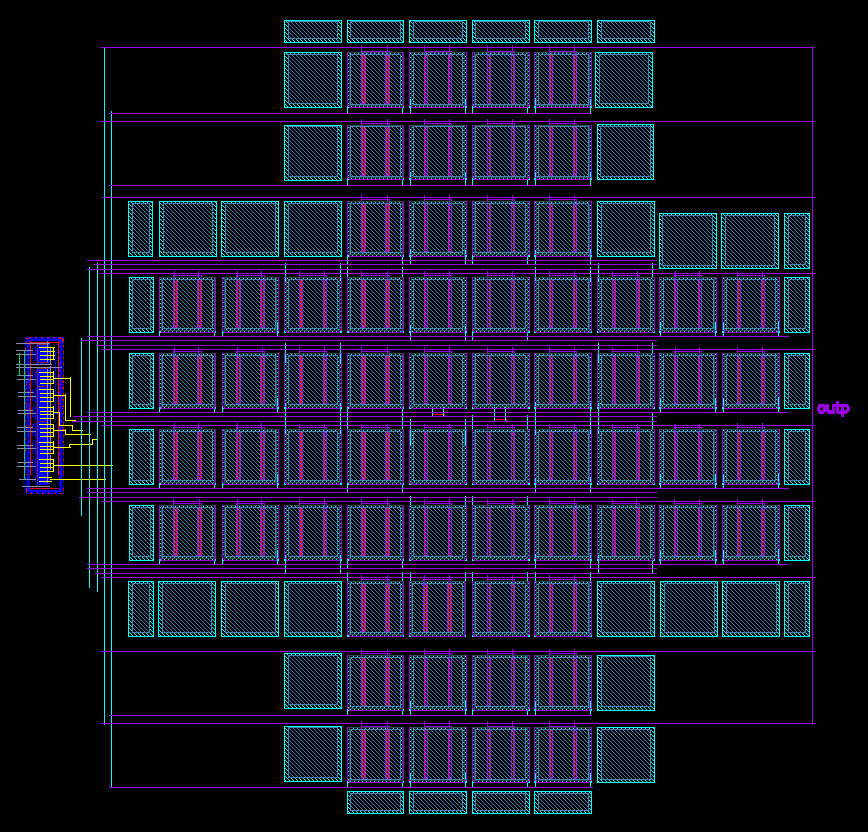
\includegraphics[height=.8\textheight]{img/cap_layout}
 \end{frame}
 
 \section{Simulations}
 \subsection{Sinusoidal Stimulus}
 \begin{frame}{Simulations I}{Sinusoidal Stimulus}
  \centering
  \tikzsetnextfilename{sinusoidal_conversion}
  \resizebox{!}{0.8\textheight}{\begin{tikzpicture}[timing/unit=0.64cm]
 \begin{axis}[
   name=analog,
   x filter/.code={\pgfmathdivide{#1}{1e-9}},
   width=\textwidth, height=0.4\textwidth,
   enlarge x limits=0,
   xlabel=\si{\ns},
   ylabel=\si{\V},
   legend cell align={left},
   grid=both, minor grid style=dotted, minor y tick num = 5, minor x tick num=3,
  ]
  \addplot [thick, red] table[x=VinX, y=VinY, col sep=comma] {./data/m3_matlab_decimated.csv};
  \addlegendentry{Input signal};
  \addplot [thick, blue] table[x=SAR_out_analogX, y=SAR_out_analogY, col sep=comma] {./data/m3_matlab_decimated.csv};
  \addlegendentry{Output signal};
 \end{axis}
 \begin{axis}[
   name=clk,
   anchor=north,
   at={($(analog.south)-(0,8ex)$)},
   width=\textwidth, height=0.17\textwidth,
   x filter/.code={\pgfmathdivide{#1}{1e-9}},
   enlarge x limits=0,
   axis line style={draw=none},
   tick style={draw=none}, ytick=\empty, xtick=\empty,
   ylabel=CLK, ylabel style={rotate=-90},
  ]

  \addplot [thick] table[x=clkX, y=clkY, col sep=comma] {./data/m3_matlab_clk.csv};
 \end{axis}
 \begin{axis}[
   name=out0,
   anchor=north,
   at={($(clk.south)-(0,2ex)$)},
   width=\textwidth, height=0.17\textwidth,
   x filter/.code={\pgfmathdivide{#1}{1e-9}},
   enlarge x limits=0,
   axis line style={draw=none},
   tick style={draw=none}, ytick=\empty, xtick=\empty,
   ylabel={out[0]}, ylabel style={rotate=-90},
  ]
  \addplot [thick] table[x=out0X, y=out0Y, col sep=comma] {./data/m3_matlab_decimated.csv};
 \end{axis}
 \begin{axis}[
   name=out1,
   anchor=north,
   at={($(out0.south)-(0,2ex)$)},
   width=\textwidth, height=0.17\textwidth,
   x filter/.code={\pgfmathdivide{#1}{1e-9}},
   enlarge x limits=0,
   axis line style={draw=none},
   tick style={draw=none}, ytick=\empty, xtick=\empty,
   ylabel={out[1]}, ylabel style={rotate=-90},
  ]
  \addplot [thick] table[x=out1X, y=out1Y, col sep=comma] {./data/m3_matlab_decimated.csv};
 \end{axis}
 \begin{axis}[
   name=out2,
   anchor=north,
   at={($(out1.south)-(0,2ex)$)},
   width=\textwidth, height=0.17\textwidth,
   x filter/.code={\pgfmathdivide{#1}{1e-9}},
   enlarge x limits=0,
   axis line style={draw=none},
   tick style={draw=none}, ytick=\empty, xtick=\empty,
   ylabel={out[2]}, ylabel style={rotate=-90},
  ]
  \addplot [thick] table[x=out2X, y=out2Y, col sep=comma] {./data/m3_matlab_decimated.csv};
 \end{axis}
 \begin{axis}[
   name=out3,
   anchor=north,
   at={($(out2.south)-(0,2ex)$)},
   width=\textwidth, height=0.17\textwidth,
   x filter/.code={\pgfmathdivide{#1}{1e-9}},
   enlarge x limits=0,
   axis line style={draw=none},
   tick style={draw=none}, ytick=\empty, xtick=\empty,
   ylabel={out[3]}, ylabel style={rotate=-90},
  ]
  \addplot [thick] table[x=out3X, y=out3Y, col sep=comma] {./data/m3_matlab_decimated.csv};
 \end{axis}
 \begin{axis}[
   name=out4,
   anchor=north,
   at={($(out3.south)-(0,2ex)$)},
   width=\textwidth, height=0.17\textwidth,
   x filter/.code={\pgfmathdivide{#1}{1e-9}},
   enlarge x limits=0,
   axis line style={draw=none},
   tick style={draw=none}, ytick=\empty, xtick=\empty,
   ylabel={out[4]}, ylabel style={rotate=-90},
  ]
  \addplot [thick] table[x=out4X, y=out4Y, col sep=comma] {./data/m3_matlab_decimated.csv};
 \end{axis}
 \draw (out4.south west) ++ (0,-7ex) coordinate (en);
 \timing at (en) {D{00}D{14}D{25}D{29}D{22}D{10}2D{00}D{03}D{15}D{26}D{28}D{22}D{10}0.5D{0}};
 \draw (en) ++ (0,2ex)node[left] {out[4:0]};
\end{tikzpicture}
}
 \end{frame}

 \subsection{Ramp Stimulus}
 \begin{frame}{Simulations II}{Ramp Stimulus}
  \centering
  \tikzsetnextfilename{ramp_conversion}
  \resizebox{!}{0.8\textheight}{\begin{tikzpicture}[timing/unit=0.257cm]
 \begin{axis}[
   name=analog,
   x filter/.code={\pgfmathdivide{#1}{1e-6}},
   width=\textwidth, height=0.4\textwidth,
   enlarge x limits=0,
   xlabel=\si{\us},
   ylabel=\si{\V},
   legend cell align={left},
   grid=both, minor grid style=dotted, minor y tick num = 5, minor x tick num=3,
   legend pos=north west,
  ]
  \addplot [thick, red] table[x=VinX, y=VinY, col sep=comma] {./data/m3_ramp.csv};
  \addlegendentry{Input signal};
  \addplot [thick, blue] table[x=SAR_out_analogX, y=SAR_out_analogY, col sep=comma] {./data/m3_ramp.csv};
  \addlegendentry{Output signal};
 \end{axis} 
 \begin{axis}[
   name=clk,
   anchor=north,
   at={($(analog.south)-(0,8ex)$)},
   width=\textwidth, height=0.17\textwidth,
   x filter/.code={\pgfmathdivide{#1}{1e-6}},
   enlarge x limits=0,
   axis line style={draw=none},
   tick style={draw=none}, ytick=\empty, xtick=\empty,
   ylabel=CLK, ylabel style={rotate=-90},
  ]
  \addplot [thick] table[x=clkX, y=clkY, col sep=comma] {./data/m3_matlab_clk.csv};
 \end{axis}
 \begin{axis}[
   name=out0,
   anchor=north,
   at={($(clk.south)-(0,1.5ex)$)},
   width=\textwidth, height=0.17\textwidth,
   x filter/.code={\pgfmathdivide{#1}{1e-6}},
   enlarge x limits=0,
   axis line style={draw=none},
   tick style={draw=none}, ytick=\empty, xtick=\empty,
   ylabel={out[0]}, ylabel style={rotate=-90},
  ]
  \addplot [thick] table[x=out0X, y=out0Y, col sep=comma] {./data/m3_ramp.csv};
 \end{axis}
 \begin{axis}[
   name=out1,
   anchor=north,
   at={($(out0.south)-(0,2ex)$)},
   width=\textwidth, height=0.17\textwidth,
   x filter/.code={\pgfmathdivide{#1}{1e-6}},
   enlarge x limits=0,
   axis line style={draw=none},
   tick style={draw=none}, ytick=\empty, xtick=\empty,
   ylabel={out[1]}, ylabel style={rotate=-90},
  ]
  \addplot [thick] table[x=out1X, y=out1Y, col sep=comma] {./data/m3_ramp.csv};
 \end{axis}
 \begin{axis}[
   name=out2,
   anchor=north,
   at={($(out1.south)-(0,2ex)$)},
   width=\textwidth, height=0.17\textwidth,
   x filter/.code={\pgfmathdivide{#1}{1e-6}},
   enlarge x limits=0,
   axis line style={draw=none},
   tick style={draw=none}, ytick=\empty, xtick=\empty,
   ylabel={out[2]}, ylabel style={rotate=-90},
  ]
  \addplot [thick] table[x=out2X, y=out2Y, col sep=comma] {./data/m3_ramp.csv};
 \end{axis}
 \begin{axis}[
   name=out3,
   anchor=north,
   at={($(out2.south)-(0,2ex)$)},
   width=\textwidth, height=0.17\textwidth,
   x filter/.code={\pgfmathdivide{#1}{1e-6}},
   enlarge x limits=0,
   axis line style={draw=none},
   tick style={draw=none}, ytick=\empty, xtick=\empty,
   ylabel={out[3]}, ylabel style={rotate=-90},
  ]
  \addplot [thick] table[x=out3X, y=out3Y, col sep=comma] {./data/m3_ramp.csv};
 \end{axis}
 \begin{axis}[
   name=out4,
   anchor=north,
   at={($(out3.south)-(0,2ex)$)},
   width=\textwidth, height=0.17\textwidth,
   x filter/.code={\pgfmathdivide{#1}{1e-6}},
   enlarge x limits=0,
   axis line style={draw=none},
   tick style={draw=none}, ytick=\empty, xtick=\empty,
   ylabel={out[4]}, ylabel style={rotate=-90},
  ]
  \addplot [thick] table[x=out4X, y=out4Y, col sep=comma] {./data/m3_ramp.csv};
 \end{axis}
 \draw (out4.south west) ++ (0,-4ex) coordinate (en);
 \timing at (en) {D{00}D{01}D{02}D{03}D{04}D{05}D{06}D{07}D{08}D{09}D{10}D{11}D{12}D{13}D{14}D{15}D{16}D{17}D{18}D{19}D{20}D{21}D{22}D{23}D{24}D{25}D{26}D{16}D{27}D{28}D{29}D{30}4D{31}};
 \draw (en) ++ (0,0.8ex)node[left] {out[4:0]};
\end{tikzpicture}
}
 \end{frame}

 \subsection{Spectrum}
 \begin{frame}{Simulations III}{Spectrum}
  \begin{center}
   \tikzsetnextfilename{spectrum}
   \begin{tikzpicture}
 \begin{axis}
  [name=en,
   width=\textwidth,
   height=0.7\textheight,
   x filter/.code={\pgfmathdivide{#1}{1e6}},
   xlabel=$f/\si{\MHz}$,
   ylabel=\si{dB},
   x label style={at={(axis description cs: 0.5,-0.1)},anchor=north},
   y label style={at={(axis description cs:-0.1, 0.5)},anchor=south},
   enlarge x limits=0,
   ymin=-99,
   grid=both, minor grid style=dotted, minor y tick num = 5, minor x tick num=3,
  ]
  \addplot[thick] table[x=X, y=Y, col sep=comma] {data/spectrum.csv};
  \draw[latex-, red] (1.395, -18.53) to[in=180, out=45] (3.6,-25) node[right] {Input frquency: \SI{1.4}{\MHz}}; 
  \draw[latex-, red] (2.791, -57.13) to[in=180, out=90] (3.6,-35) node[right] {First harmonic: \SI{2.8}{\MHz}}; 
  \draw[latex-, red] (0,-18.53) to[in=180, out=0] (0.6,-25) node[right] {DC};%($V\subb{cm}$)};
 \end{axis}
 \draw (en.south west) ++(0,-1.5) node[right] {$V\subb{in},V\subb{cm} = \SI{250}{\mV}\rightarrow\SI{-12.7}{dB}$};
\end{tikzpicture}

  \end{center}
 \end{frame}
 \AtBeginSection[]{}
 
 \section{Figures of Merit}
 \begin{frame}{Figures of Merit}
  \centering
  \begin{tabular}[]{cc}
   \toprule
   Sample rate      & \SI{14.29}{\MHz}\\
   Resolution       & 5 bits\\
   Full scale       & \SI{500}{\mV}\\
   $V\subb{ref}$    & \SI{500}{\mV}\\
   $V\subb{cm}$     & \SI{250}{\mV}\\
   $V\subb{LSB}$    & \SI{15.63}{\mV}\\\midrule
   ENOB             & \num{4.78}\\
   SNDR             & \SI{30.55}{dB}\\
   SFDR             & \SI{38.16}{dB}\\
   THD              & \SI{1.44}{\percent}\\
   INL              & \alert{\SI{10.22}{\mV}}\\
   DNL              & \alert{\SI{8.32}{\mV}}\\
   Energy per cycle & \SI{4.02}{\pico\joule}\\\bottomrule
  \end{tabular}
 \end{frame}
 \section{Conclusions}
 \begin{frame}{Conclusions}
  We were able to:\vspace*{2em}
  \begin{itemize}
   \item Work on a state-of-the-art ADC topology
   \item<2-> Learn behavioral modeling techniques
   \item<3-> Hands-on experience with charge redistribution circuits
   \item<4-> Gained knowledge about mixed-signal design and simulations
  \end{itemize}
 \end{frame}

 \section{References}
 \begin{frame}{References}
  \begin{thebibliography}{9}
   \setbeamertemplate{bibliography item} [article]
   \bibitem{C} A. Rusu, {\textit{IL2238 \& IL2239 Lecture Slides}}, KTH 2018.
   \bibitem{D} N. Ivanisevic, P. Chaourani, M. Waqar and D. I. Albertsson, \textit{{Course Tutorials}}, KTH 2018.
   \setbeamertemplate{bibliography item} [book]
   \bibitem{A} T.C. Carusone, D. Johns and K. Martin, {\textit{Analog Integrated Circuit Design}}, Wiley 2011.
   \bibitem{B} C. Saint and J. Saing, {\textit{IC Mask Design: Essential Layout Techniques}}, McGraw-Hill Professional Engineering 2002.
   \bibitem{C} B. Razavi, \textit{Principles of Data Conversion System Design}, Wiley 1995.
  \end{thebibliography}
 \end{frame}
\end{document} 
